
\subsection{The straightforward approach}

The first attempt was quite straightforward and a little bit explorative in the way that the author had to discover the MPS API that allows programmatical language generation. Because MPS is still in development, the API isn't that well documented and some features had to be discovered through trial and error or by examination of the PE4MPS project (\ref{chap:pe4mps}) which served a great aid here. Another big topic here was how to split the code and whether to use only MPS for writing the BaseLang code that will be compiled into Java, or whether to create separate Java projects and use other tools because creating a large volume of BaseLang code in MPS isn't always a comfortable experience. We will talk about this further down in chapter [TODO: chapter reference].

\subsubsection{The algorithm}
The main idea behind the first attempt comes from the realization, that when a parser rules breaks into more alternatives, for example like the \parserrule{content} rule:

\begin{antlr}
	\parserrule{content}    :   \lexerrule{TEXT}
           |   \parserrule{element}
           |   \parserrule{comment}
           |   \lexerrule{CDATA}
           ;
\end{antlr}  

We will need to have 4 elements that are somehow marked as belonging to this parser rule. That is why we decided, that for each rule with more than one alternative, we will create an interface concept. Then for each alternative of this rule, we will create a classic concept that will implement this interface. So for our \parserrule{content} example, we will get following setup:

\begin{antlr}
	\interface{IContent}   :   \concept{Content_1}
           |   \concept{Content_2}
           |   \concept{Content_3}
           |   \concept{Content_4}
\end{antlr}

When the \parserrule{content} parser rule is then referenced inside some alternative (e.g. first alternative of the \parserrule{element} rule), we will set the \interface{IContent} interface as the child instead and all of the four implementors can be assigned to this child. For rules with a single alternative, no interface is needed. For rules that contain inline block rules, we have already created artificial rules in our tree representation that we generated in the parser stage which means they have already been taken care of.

\subsubsection{The layer problem}

This simple algorithm will leave us with an MPS language that follows given structure correctly and could be used to represent code in that language inside MPS (coding will not be possible as there is no editor aspect defined yet). There is one problem, however, concerning usability of such language. We will demonstrate this problem on the SimpleXML language, using \parserrule{element} and \parserrule{content} rules:

\begin{antlr}
	\parserrule{content}    :   \lexerrule{TEXT}
           |   \parserrule{element}
           |   \parserrule{comment}
           |   \lexerrule{CDATA}
           ;
	
	\parserrule{element}    :   \literal{<} \lexerrule{Name} \parserrule{attribute}* \literal{>} \parserrule{content}* \literal{</} \lexerrule{Name} \literal{>}
           |   \literal{<} \lexerrule{Name} \parserrule{attribute}* \literal{/>}
           ;	
\end{antlr} 

When we would be coding in this language, the MPS auto-complete would give us aid when filling out all properties and children of inserted concepts. Imagine there is a freshly inserted \concept{Element{\_}1} concept (a concept representing the full XML element as is stated in the first alternative of the \parserrule{element} parser rule). Now we would like to insert some content inside. Let's say we would like to insert another XML element inside. We would place cursor in the content placeholder and press Ctrl+Space to view the auto-completion options.
\\

Following the algorithm mentioned above, we have created a child of the \concept{Element{\_}1} concept of type \interface{IContent}. There exist four concepts which implement the \interface{IContent} interface. MPS evaluated this and gave us four options inside the auto-complete. This auto-complete is captured in figure \ref{fig:layer_problem}.

\begin{figure}[h]
	\centering
	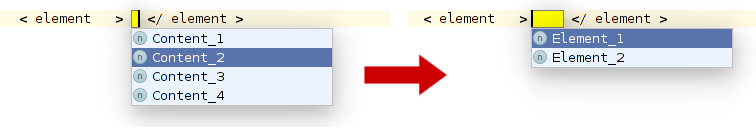
\includegraphics[width=\textwidth]{../img/layer_problem.png}
	\caption{Layer problem in auto-completion}
	\label{fig:layer_problem}
\end{figure}

In order to correctly insert another nested element inside, we would have to first insert a \concept{Content{\_}2} concept inside \concept{Element{\_}1} that has an \interface{IElement} child inside (and nothing else). Then, as a second step we would call for the auto-complete again and insert either \concept{Element{\_}1} or \concept{Element{\_}2} inside \concept{Content{\_}2}. This mean that we have to go through two steps and in the first one either guess or remember the grammar rule's alternative order, to know which option we should go with in the first step. And the problem goes both ways - if we decide to replace the nested \concept{Element{\_}1} with let's say an XML comment (a \concept{Comment} concept), we need to delete both intermediary layers before we get back to the original \concept{Content{\_}X} crossroads. Meanwhile the user cannot really see what is happening since the intermediary level has no appearance or indicator. This leads to a confusion of the user.
\\

We tried to ease this situation up by creating aliases for concepts derived from their content (names such as “Element content” or “CDATA content” instead of \concept{Content{\_}N)}, but the problem goes beyond this. Take into consideration that the SimpleXML grammar is a very simple one. More sophisticated languages may have more than two intermediary layers and writing code would consist of clicking through a large number of auto-completes like shown in the example above. There is also nothing preventing authors of grammars from naming these helper layers in a completely unrelated manner, which would make user's orientation even harder. After all, these layers come into existence when the grammar is being written so that it is more readable for humans and maybe better maintainable by the author. It has nothing to do with making the AST simple for the ANTLR parser. ANTLR is very capable and handles this probably very well in any form. 
\\

Furthermore, using inline block rules makes this even bigger problem as the block rules' names are auto-generated by our parser and differ only by numbers, even though the alias assigning process improves the situation by a bit. But from the point of view of the grammar's author, it is an invisible layer of rules nested inside.
\\

For better illustration, we have put examples of languages, that were generated by this algorithm, on the attached DVD. The reader can try them out on their own and see for themselves that this makes the language very unfriendly and hard to use.
